\chapter{Introduction non facultative}\label{chapIntro}

Ce chapitre présente les besoins et les concepts de la gestion de
version d'une manière générale, ainsi qu'un aperçu des différentes
familles de systèmes de gestion de version. Il se focalise ensuite sur
Git, qui sera l'objet du reste de cet ouvrage, pour en expliquer la
philosophie et le modèle de fonctionnement.

\section{Les besoins du génie logiciel}

La \textbf{gestion de versions}\index{Gestion de versions} (en anglais
\textit{version control} ou \textit{revision control}) est une
fonctionnalité, ou plutôt une famille de fonctionnalités, qui trouve
son origine dans les besoins du développement logiciel en
équipe. Plusieurs développeurs travaillant ensemble sur le même
ensemble de fichiers, même si les domaines d'intervention de chacun
sont clairement définis, doivent nécessairement trouver un moyen de
collaborer de manière constructive, sans que les contributions des uns
ne deviennent un souci pour les autres. La gestion de version, en
s'appuyant sur un \textbf{historique}\index{historique} raisonné du
développement, a pour vocation de répondre à l'ensemble des besoins
détaillés ci-après.

\subsection{Gestion des instances du projet}

Les outils de gestion de versions doivent permettre d'identifier
plusieurs instances (éventuellement à des stades de développement
différents) du même projet. Ces instances peuvent correspondre,
suivant les cas, à l'espace de travail direct d'un développeur ou d'un
ensemble de développeur, à une instance de référence commune partagée
par l'ensemble ou un sous-ensemble des développeurs, à une instance de
publication des versions stables du projet\ldots

Ces instances sont désignées sous le terme générique de
\textbf{dépôt}\index{depot@dépôt} (\textit{repository} en
anglais). Chaque dépôt est une représentation du projet. Suivant les
choix d'organisation et le système de gestion de versions utilisé, un
dépôt peut représenter le projet dans son intégralité ou bien
seulement un sous-ensemble, l'intégralité de son historique ou bien
seulement une partie. Un dépôt peut être
\textbf{local}\index{depot@dépôt!local}, c'est-à-dire situé surl la
machine de développement d'un des contributeurs (sans être
nécessairement confondu avec l'espace de travail direct du
développeur), ou bien \textbf{distant}\index{depot@dépôt!distant},
déporté sur un serveur accessible via le réseau.

\subsection{Gestion de l'historique}

La gestion de versions est un moyen de conserver une trace de
l'historique du projet, sous la forme d'un ensemble de
\textbf{révisions}\index{revision@révision} (\textit{commits} en
anglais). Une révision est un ensemble atomique et identifiable de
modifications liées par une certaine unité sémantique, portant sur un
ou plusieurs fichiers, réalisées par un même contributeur identifié,
explicitement introduites dans le projet accompagnées d'un message
explicatif et d'autres méta-données, comme la date\footnote{Dans
  certains systèmes, comme par exemple Overleaf\index{Overleaf}, qui
  est une surcouche web de Git pour la rédaction collaborative
  (\url{https://www.overleaf.com/}), les révisions peuvent être
  générées automatiquement, de manière périodique ou à chaque
  modification élémentaire. Dans ce cas, une révision peut n'avoir ni
  unité sémantique ni message explicatif, ce qui limite forcément
  l'utilité de l'historique correspondant. D'autre part, l'unicité
  sémantique des révisions est une propriété qui, si elle est
  désirable, dépend en grande partie de la bonne volonté des
  contributeurs\ldots}. L'atomicité signifie que les modifications
d'une même révision sont toutes appliquées ensemble au projet (ou
qu'aucune ne l'est), sans qu'une modification provenant d'une autre
révision puisse venir interférer ni que le projet puisse se retrouver
dans un état incohérent (avec une révision partiellement
appliquée)\footnote{Il existe des systèmes de gestion de versions dans
  lesquels les révisions ne sont pas atomiques. Nous ne les
  mentionneront pas ici dans l'espoir que leur nom disparaisse à
  jamais de la mémoire collective et de l'histoire de l'informatique
  (pour plus de détails sur les bonnes pratiques du révisionnisme avec
  Git, les nostalgiques du Ministère de la Vérité \cite{Orwell}
  pourront étudier avec intérêt la section~\ref{secRevisionnisme}).}.
Par abus de langage, le terme de révision ou de \textit{commit}
désigne également l'état du projet après application des modifications
en question.

Dans le cas le plus simple, un historique est une succession linéaire
de révisions, chacune s'appuyant sur la précédente
(figure~\ref{fig:historiqueLineaire}). Dans la majorité des cas,
cependant, il en ira tout autrement\ldots Dans la syntaxe graphique
que nous adoptons pour les historiques, les cercles représentent les
révisions et les flèches représentent les dépendances entre
ces révisions. Le sens de ces flèches n'est donc pas le sens d'écoulement
du temps (qui va de la gauche vers la droite pour un historique
linéaire)~: le fait que la révision $E$ pointe vers la révision $D$
($D \leftarrow E$) veut dire que $E$ s'appuie sur $D$, et donc qu'elle
vient après cette dernière dans le processus de conception.

\begin{figure}[h!]
  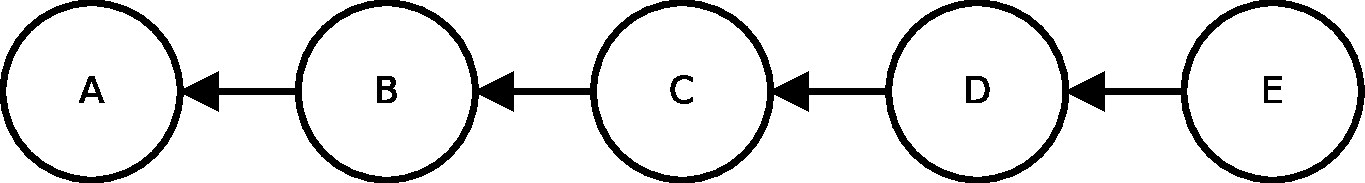
\includegraphics[width=10cm]{figures/historiqueLineaire}
  \caption{Exemple d'historique de développement linéaire, constitué
    de cinq révisions successives.\label{fig:historiqueLineaire}}
\end{figure}


L'historique a lui-même différentes utilités, au-delà de ce rôle de
représentation temporelle, notamment parce qu'il est généralement
navigable, voire cherchable. Suivant les systèmes, l'historique peut
permettre de déterminer~:
\begin{itemize}
\item La date d'introduction d'une révision donnée~;
\item L'auteur d'une révision donnée~;
\item Les modifications apportées par une révision donnée~;
\item Les causes et motivations d'une modification (si la révision
  concernée a été correctement documentée)~;
\item La révision ayant introduit une fonctionnalité, un
  bogue\index{bogue}, une régression\index{regression@régression}, une
  vulnérabilité\ldots
\end{itemize}

\subsection{Intégration de contributions dans un même projet} % TODO 

Les différentes personnes participant à un même projet doivent pouvoir
voir leurs contributions individuelles intégrées au projet, idéalement
de manière fluide, transparente et indolore.

Intégration des contributions de différentes personnes dans un
  même projet, en permettant la résolution des incohérences pouvant
  survenir entre des modifications concurrentes~;

% Développement de fonctionnalités en parallèle, fusion, résolution de conflits
% Notion de conflit
\index{conflit}


\subsection{Gestion de variantes différentes du même projet} % TODO 

Possibilité de créer et de maintenir simultanément des variantes du
projet, par exemple pour expérimenter l'utilisation de nouvelles
technologies, le développement de nouvelles fonctionnalités ou la mise
en place d'une nouvelle organisation~;

\section{Systèmes de gestion de version} %TODO
\index{systeme de gestion de versions@système de gestion de versions}

% fichiers texte et fichiers binaires

\subsection{Systèmes centralisés} %TODO
\index{systeme de gestion de versions@système de gestion de versions!centralises@centralisé}
% TODO CVS
\index{CVS}
% TODO Subversion
\index{Subversion}
% TODO Visual SourceSafe
\index{Visual SourceSafe}
% TODO Perforce Helix
\index{Perforce Helix}
% TODO VSTS (Visual Studio Team Services)
\index{Visual Studio Team Services}

\subsection{Systèmes décentralisés} %TODO
\index{systeme de gestion de versions@système de gestion de versions!decentralises@décentralisé}
% TODO Git
\index{Git}
% TODO GNU arch
\index{GNU arch}
% TODO Mercurial
\index{Mercurial}
% TODO BitKeeper
\index{BitKeeper}
% TODO Bazaar
\index{Bazaar}
% TODO Darcs
\index{Darcs}
% TODO Veracity
\index{Veracity}
% TODO VSTS (Visual Studio Team Services)
\index{Visual Studio Team Services}

\section{Le modèle de Git} %TODO
% TODO philosophie, différents éléments du modèle

\subsection{Principes et philosophie} %TODO

\subsection{Git sur les différents systèmes d'exploitation}\label{GitOS} %TODO
\index{Windows}
\index{Linux}
\index{macOS}

\subsection{Les différents éléments du modèle} %TODO

\index{.git@\texttt{.git}}

\index{SHA1}
% TODO Expliquer en footnote que Git utilise SHA1 comme un code de
% détection d'erreur et non comme un algorithme de hachage
% cryptographique. En théorie, il est possible de falsifier le contenu
% d'un commit Git utilisant SHA1, par exemple pour y insérer du code
% malveillant, en conservant le même haché. Subversion utilise SHA1
% également, et les PDF en collision le faisaient planter, nécessitant
% un correctif. Sauf que Git utilise également SHA1 pour signer les
% commits, et là évidemment ça pose un problème d'authenticité et plus
% seulement d'intégrité.
% http://www.zdnet.fr/actualites/collision-sha-1-linus-torvalds-se-veut-rassurant-sur-git-39849070.htm
% https://twitter.com/matthew_d_green/status/835864260240683009/photo/1

\subsection{Structure d'un dépôt} %TODO
\index{depot@dépôt}
\index{depot@dépôt!local}
% TODO notion de référence

\subsection{Modèle de configuration} %TODO
\index{configuration}
\index{git@\texttt{git}!config@\texttt{config}}
\index{global@\texttt{global}}
\index{system@\texttt{system}}
\index{local@\texttt{local}}
% TODO global / system / local, principales variables